\documentclass[10pt,twocolumn,twoside,slovak,a4paper]{article}

\usepackage[slovak]{babel}
\usepackage[T1]{fontenc}
\usepackage[utf8]{inputenc}

\usepackage{graphicx}
\usepackage{amsmath}
\usepackage{wrapfig}
\usepackage{url}
\usepackage{hyperref}
\usepackage{cite}

\title{Prehľadový článok}
\author{Yasin Cikkel}
\date{6. október 2026}

\begin{document}

\maketitle

\begin{abstract}
Toto je predbežná verzia prehľadového článku.
Dokument obsahuje ukážky práce s diagramami, obrázkami,
zoznamami a matematickými výrazmi v prostredí LaTeX.
\end{abstract}


\section{Úvod}
\label{uvod}

Táto časť predstavuje úvod do problematiky.
Cieľom článku je ukázať základnú štruktúru dokumentu
a možnosti práce s rôznymi prvkami v LaTeXu.


\section{Logo FIIT STU}
\label{logo}

\begin{wrapfigure}{r}{0.22\textwidth}
    \centering
    
\includegraphics[width=0.20\textwidth]{images.png}
\end{wrapfigure}

Logo FIIT STU je vložené ako plávajúci obrázok.
Text ho obteká z ľavej strany. Takýmto spôsobom možno vhodne
umiestniť logo alebo iný menší obrázok priamo do textu bez toho,
aby sa prerušil tok dokumentu. Text pokračuje ďalej vedľa obrázka,
a po skončení jeho výšky sa opäť rozšíri na celú šírku stĺpca.


\section{Iná časť}
\label{ina}

Základným problémom je teda\ldots{}
Najprv sa pozrieme na nejaké vysvetlenie
(časť~\ref{ina:nejake}) a potom na ďalšie vysvetlenie
(časť~\ref{ina:este}).

\footnote{Niekedy môžete potrebovať aj poznámku pod čiarou.}

Môže sa zdať, že problém vlastne nejestvuje~\cite{Coplien:MPD},
ale bolo dokázané, že to tak nie je~\cite{Czarnecki:Staged,Czarnecki:Progress}.

Dôležité veci možno \emph{zdôrazniť kurzívou}.


\subsection{Nejaké vysvetlenie}
\label{ina:nejake}

Nasledujúce dva diagramy sú zobrazené vedľa seba:

\begin{figure*}[t]
    \centering

    \begin{minipage}{0.47\textwidth}
        \centering
        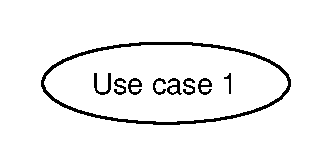
\includegraphics[width=\linewidth]{grafika.pdf}
    \end{minipage}
    \hfill
    \begin{minipage}{0.47\textwidth}
        \centering
        
\includegraphics[width=\linewidth]{diagram2.pdf}
    \end{minipage}

    \caption{Dva diagramy vedľa seba}
    \label{fig:dva_diagramy}
\end{figure*}


\section{Obrázok cez oba stĺpce}
\label{obrazok_cez_stlpce}

Nasledujúci obrázok je vložený cez oba stĺpce dvojstĺpcového dokumentu.

\begin{figure*}[t]
    \centering
    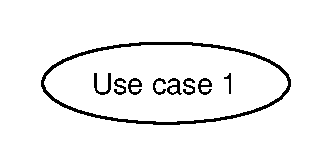
\includegraphics[width=0.80\textwidth]{grafika.pdf}
    \caption{Obrázok zobrazený cez oba stĺpce}
    \label{fig:cez_obidva_stlpce}
\end{figure*}


\subsection{Zoznam}
\label{zoznam}

Niekedy treba uviesť zoznam:

\begin{itemize}
    \item jedna vec
    \item druhá vec
    \begin{itemize}
        \item x
        \item y
    \end{itemize}
\end{itemize}

Ten istý zoznam, len číslovaný:

\begin{enumerate}
    \item jedna vec
    \item druhá vec
    \begin{enumerate}
        \item x
        \item y
    \end{enumerate}
\end{enumerate}


\subsection{Ešte nejaké vysvetlenie}
\label{ina:este}

\paragraph{Veľmi dôležitá poznámka.}
Niekedy je potrebné nadpisom označiť odsek.
Text pokračuje hneď za nadpisom.


\section{Matematická ukážka}
\label{matematika}

Nasledujúca matica má rozmery $5 \times 4$:

\[
A =
\begin{pmatrix}
1 & 2 & 3 & 9 \\
5 & 6 & 7 & 8 \\
9 & 10 & 11 & 12 \\
13 & 14 & 15 & 16 \\
17 & 18 & 19 & 20
\end{pmatrix}
\]

Ukážka dlhšieho matematického výrazu:

\[
a_n =
a_1 + (n-1)d
+ \frac{n(n-1)}{2}
+ \frac{n(n-1)(2n-1)}{6}
\]


\section{Dôležitá časť}
\label{dolezita}

Sem môžete doplniť obsah dôležitej časti článku.


\section{Ešte dôležitejšia časť}
\label{dolezitejsia}

Sem môžete doplniť obsah ďalšej dôležitej časti článku.


\section{Záver}
\label{zaver}

V závere stručne zhrňte hlavné poznatky článku.


\bibliographystyle{plain}
\bibliography{literatura}

\end{document}